\documentclass[aspectratio=169, 11pt]{beamer}
% \documentclass[aspectratio=169, 11pt, handout]{beamer}

% ── Theme ──
\usetheme{Madrid}
\usecolortheme{default}
\setbeamertemplate{navigation symbols}{}
\setbeamertemplate{footline}{%
  \leavevmode\hbox{%
    \begin{beamercolorbox}[wd=.333333\paperwidth,ht=2.5ex,dp=1ex,center]{author in head/foot}%
      \usebeamerfont{author in head/foot}\insertshortauthor
    \end{beamercolorbox}%
    \begin{beamercolorbox}[wd=.333333\paperwidth,ht=2.5ex,dp=1ex,center]{title in head/foot}%
      \usebeamerfont{title in head/foot}\insertshorttitle
    \end{beamercolorbox}%
    \begin{beamercolorbox}[wd=.333333\paperwidth,ht=2.5ex,dp=1ex,right]{date in head/foot}%
      \usebeamerfont{date in head/foot}\insertframenumber{} / \inserttotalframenumber\hspace*{2ex}
    \end{beamercolorbox}}}

% ── Packages ──
\usepackage{amsmath,amssymb}
\usepackage{booktabs}
\usepackage{xcolor}
\usepackage{colortbl}
\usepackage{tikz}
\usetikzlibrary{arrows.meta, positioning}
\usetikzlibrary{calc} 

% ── Colors ──
\definecolor{sbgreen}{HTML}{00704A}
\definecolor{warnred}{HTML}{CC0000}
\definecolor{noteblue}{HTML}{2060A0}

% ── Commands ──
\newcommand{\E}{\mathbb{E}}
\newcommand{\Var}{\mathrm{Var}}
\newcommand{\Cov}{\mathrm{Cov}}
\newcommand{\SE}{\mathrm{SE}}
\newcommand{\Prob}{\mathrm{Pr}}
\newcommand{\indep}{\perp\!\!\!\perp}
\DeclareMathOperator{\plim}{plim}

% ── Title ──
\title[Lecture 4]{Lecture 4: Model Evaluation}
\subtitle{Applied ML for Business Part II}
\author{Zhikun Lu}
\date{\today}


\begin{document}

% ====================================================================
\begin{frame}
\titlepage
\end{frame}

% ====================================================================
\begin{frame}{Where We Are}

\begin{center}
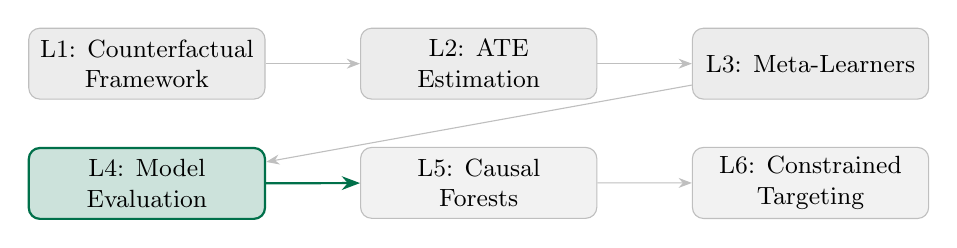
\begin{tikzpicture}[
    node distance=0.6cm and 1.2cm,
    box/.style={draw, rounded corners, minimum width=3cm, minimum height=0.9cm, font=\small, align=center},
    done/.style={box, fill=gray!15, draw=gray!50},
    active/.style={box, fill=sbgreen!20, draw=sbgreen, thick},
    inactive/.style={box, fill=gray!10, draw=gray!50}
]
\node[done] (L1) {L1: Counterfactual\\Framework};
\node[done, right=of L1] (L2) {L2: ATE\\Estimation};
\node[done, right=of L2] (L3) {L3: Meta-Learners};
\node[active, below=of L1] (L4) {L4: Model\\Evaluation};
\node[inactive, below=of L2] (L5) {L5: Causal\\Forests};
\node[inactive, below=of L3] (L6) {L6: Constrained\\Targeting};

\draw[-{Stealth}, gray!50] (L1) -- (L2);
\draw[-{Stealth}, gray!50] (L2) -- (L3);
\draw[-{Stealth}, gray!50] (L3) -- (L4);
\draw[-{Stealth}, thick, sbgreen] (L4) -- (L5);
\draw[-{Stealth}, gray!50] (L5) -- (L6);
\end{tikzpicture}
\end{center}
\end{frame}

% ====================================================================
\begin{frame}{The Targeting Depth Curve}
 
Rank all customers by $\hat{\tau}(x_i)$ descending. As we expand the target set, the ATT falls:
 
\bigskip
 
\begin{center}
\begin{tabular}{lccc}
\toprule
\textbf{Depth} $k$ & \textbf{Who is targeted} & $\tau_{S_k}$ & \textbf{Interpretation} \\
\midrule
1,000 & Top 1,000 analysts & 0.20 & Highest-effect only \\
5,000 & All analysts & 0.20 & All high-effect customers \\
7,500 & Analysts $+$ 2,500 exec & 0.15 & Diluted by executives \\
10,000 & Everyone & 0.125 & $=$ ATE \\
\bottomrule
\end{tabular}
\end{center}
 
\bigskip
 
If the ranking is corrupted (noisy, biased), we treat the wrong people and $\tau_{S_k}$ is lower at every depth.
\end{frame}
 
% ====================================================================
\begin{frame}{Ranking Quality Is What Matters}
 
Sometimes, the business value of CATE estimation depends on how well $\hat{\tau}(x)$ \emph{ranks} customers, not on the accuracy of individual point estimates.
 
\bigskip
 
A model with correct rankings but wrong magnitudes produces a better targeting rule than a model with accurate magnitudes but poor rankings.
 
\bigskip
 
$\Rightarrow$ We need an \textbf{evaluation framework} for CATE rankings.
 
\end{frame}

% %%%%%%%%%%%%%%%%%%%%%%%%%%%%%%%%%%%%%%%%%%%%%%%%%%%%%%%%%%%%%%%%%%%%
% SESSION 2: UPLIFT EVALUATION
% %%%%%%%%%%%%%%%%%%%%%%%%%%%%%%%%%%%%%%%%%%%%%%%%%%%%%%%%%%%%%%%%%%%%
 
% ====================================================================
\section{Uplift Evaluation}
% ====================================================================
 
\begin{frame}{Roadmap}
 
\textbf{Model Evaluation} 
\begin{enumerate}
    \item The evaluation problem
    \item Qini curves and AUUC
    \item RATE: formal inference for model comparison
    \item Calibration
    \item Policy value estimation
    \item Honest evaluation via sample splitting
\end{enumerate}

\end{frame}
 
% ====================================================================
\begin{frame}{The Evaluation Problem}
 
\textbf{Standard ML:} Compare predictions to observed labels.
\begin{itemize}
    \item Accuracy, AUC, RMSE, \ldots
    \item Ground truth exists for every observation
\end{itemize}
 
\bigskip
 
\textbf{Causal ML:} The \emph{label} $\tau_i = Y_i(1) - Y_i(0)$ is \textbf{never observed}.
 
\begin{itemize}
    \item We see $Y_i(1)$ or $Y_i(0)$, never both $\Longrightarrow$ ground truth $\tau_i$ never known
    \item Cannot compute $\frac{1}{n}\sum_i (\hat{\tau}(x_i) - \tau_i)^2$
\end{itemize}
 
\bigskip
 
\begin{alertblock}{Key Insight}
Evaluate the \textbf{quality of the targeting decisions}, not the accuracy of point estimates. Use \textbf{group-level} experimental comparisons.
\end{alertblock}
\end{frame}
 
% ====================================================================
\begin{frame}{The Thought Experiment}
 
Suppose a model ranks customers by $\hat{\tau}(x_i)$ from highest to lowest.
 
\bigskip
 
\textbf{Question:} If we send coupons to the top $k\%$ of customers, what is the treatment effect in that group?
 
\bigskip
 
\textbf{A good model should:}
\begin{itemize}
    \item Put high-CATE customers at the top $\Rightarrow$ large effect in top group
    \item Put low/negative-CATE customers at the bottom $\Rightarrow$ small or negative effect
\end{itemize}
 
\bigskip
 
\textbf{A random ranking:} the effect in the top $k\%$ equals the ATE regardless of $k$. This gives us a \textbf{baseline}.
\end{frame}
 
% ====================================================================
\begin{frame}{The Qini Curve}
 
For each fraction $\phi \in [0, 1]$ of customers targeted (ranked by $\hat{\tau}$), plot the cumulative gains:
 
\begin{center}
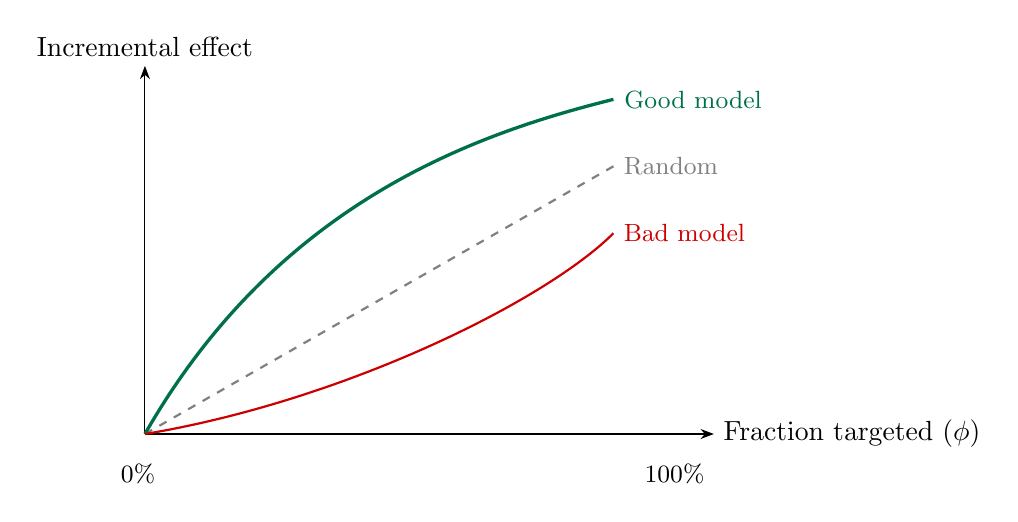
\begin{tikzpicture}[scale=0.85]
% Axes
\draw[-{Stealth}] (0,0) -- (8.5,0) node[right] {Fraction targeted ($\phi$)};
\draw[-{Stealth}] (0,0) -- (0,5.5) node[above] {Incremental effect};
 
% Random baseline (straight line)
\draw[gray, dashed, thick] (0,0) -- (7,4) node[right, font=\small] {Random};
 
% Good model (concave)
\draw[sbgreen, very thick] (0,0) .. controls (2,3.5) and (5,4.5) .. (7,5) node[right, font=\small, text=sbgreen] {Good model};
 
% Bad model (convex)
\draw[warnred, thick] (0,0) .. controls (3,0.5) and (6,2) .. (7,3) node[right, font=\small, text=warnred] {Bad model};
 
% Labels
\node[font=\small] at (4, -0.6) {0\% \hspace{6cm} 100\%};
\end{tikzpicture}
\end{center}
 
A good model: steep rise initially (high-CATE customers treated first), then flattens.
\end{frame}
 
% ====================================================================
\begin{frame}{Estimating the Qini Curve from Experimental Data}
 
We have an A/B test with treatment and control groups.
 
\bigskip
 
\textbf{Algorithm:}
\begin{enumerate}
    \item Score all customers with $\hat{\tau}(x_i)$
    \item Sort by $\hat{\tau}(x_i)$ descending
    \item For each top-$\phi$ group, compute:
    \[
    \hat{Q}(\phi) = \phi \left(\bar{Y}_1^{(\phi)} - \bar{Y}_0^{(\phi)}\right)
    \]
\end{enumerate}
 
\bigskip
 
\textbf{Why this works:} treatment assignment is random, so $\bar{Y}_1 - \bar{Y}_0$ is unbiased for the ATE \emph{within each subgroup}.
 
\bigskip
 
The model is only used for \textbf{ranking}. The experimental data provides the effect estimates.
\end{frame}
 
% ====================================================================
\begin{frame}{AUUC: Area Under the Uplift Curve}
 
\begin{block}{AUUC}
\[
\text{AUUC} = \int_0^1 \bigl[Q(\phi) - \phi \cdot \text{ATE}\bigr] \, d\phi
\]
\end{block}
 
\bigskip
 
\begin{itemize}
    \item AUUC $> 0$: model is better than random targeting
    \item AUUC $= 0$: model is no better than random
    \item AUUC $< 0$: model is worse than random (inverted ranking)
\end{itemize}
 
\bigskip
 
\textbf{Analogy:} AUUC is to CATE evaluation what AUC-ROC is to classification.
\end{frame}
 
% ====================================================================
\begin{frame}{Comparing Models with Qini Curves}
 
\begin{center}
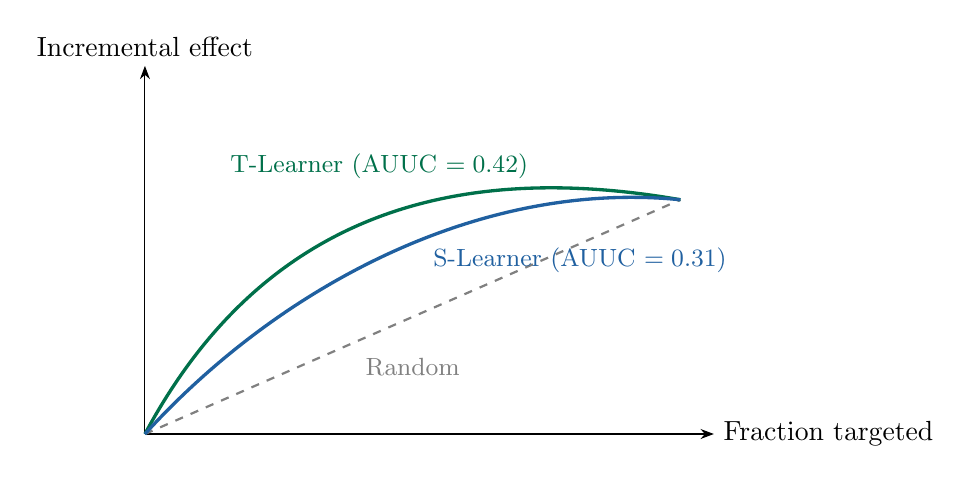
\begin{tikzpicture}[scale=0.85]
% Axes
\draw[-{Stealth}] (0,0) -- (8.5,0) node[right] {Fraction targeted};
\draw[-{Stealth}] (0,0) -- (0,5.5) node[above] {Incremental effect};
 
% Random baseline
\draw[gray, dashed, thick] (0,0) -- (8,3.5);
 
% T-Learner
\draw[sbgreen, very thick] (0,0) .. controls (1.5,2.8) and (4,4.2) .. (8,3.5);
\node[sbgreen, font=\small] at (3.5, 4.0) {T-Learner (AUUC $= 0.42$)};
 
% S-Learner
\draw[noteblue, very thick] (0,0) .. controls (2,2.2) and (5,3.8) .. (8,3.5);
\node[noteblue, font=\small] at (6.5, 2.6) {S-Learner (AUUC $= 0.31$)};
 
\node[gray, font=\small] at (4,1.0) {Random};
\end{tikzpicture}
\end{center}
 
\bigskip
 
Higher Qini curve $=$ better prioritization of high-CATE customers.
 
\bigskip
 
\textbf{But is the difference meaningful or noise?}
\end{frame}
 
% ====================================================================
\begin{frame}{RATE: Formal Inference for Model Comparison}
 
The \textbf{Rank-Weighted Average Treatment Effect} (Yadlowsky et al., 2021):
 
\begin{block}{RATE}
\[
\Theta = \frac{\Cov\bigl[\alpha(R_i),\; \tau(X_i)\bigr]}{\Var\bigl[\alpha(R_i)\bigr]}
\]
where $R_i$ is the rank of customer $i$ under $\hat{\tau}$, and $\alpha(\cdot)$ is a weighting function.
\end{block}
 
\bigskip
 
\textbf{Key property:} $\hat{\Theta}$ is asymptotically normal.
 
\bigskip
 
$\Rightarrow$ Test $H_0: \Theta = 0$ (model ranks no better than random).
 
$\Rightarrow$ Confidence intervals for comparing two models.
\end{frame}
 
% ====================================================================
\begin{frame}{RATE: Weighting Functions}
 
\textbf{TOC weight:} $\alpha(u) = \mathbf{1}(u \geq 1 - q)$
 
\begin{itemize}
    \item Average effect in the top-$q$ fraction
    \item A single point on the Qini curve
\end{itemize}
 
\bigskip
 
\textbf{AUTOC weight:} $\alpha(u) = u$
 
\begin{itemize}
    \item Smooth summary across the full ranking
    \item Normalized version of the AUUC
\end{itemize}
 
\bigskip
 
\textbf{In R:} \texttt{grf::rank\_average\_treatment\_effect()}.
 
\bigskip
 
\textbf{Practical value:} two models have AUUC of 0.018 and 0.014. Is the difference meaningful? The RATE provides a $p$-value.
\end{frame}
 
% ====================================================================
\begin{frame}{Calibration: Rankings Are Not Enough}
 
AUUC and RATE evaluate \textbf{ranking quality}. They say \textbf{nothing about magnitudes}.
 
\bigskip
 
A model predicting $\hat{\tau}(x) \in \{10, 20\}$ when true effects are $\tau(x) \in \{1, 2\}$ would rank perfectly but overstate effects by 10$\times$.
 
\bigskip
 
\textbf{Why this matters:} a marketing team projecting campaign ROI needs correct magnitudes, not just correct rankings.
\end{frame}
 
% ====================================================================
\begin{frame}{The CATE Reliability Diagram}
 
\textbf{Procedure:}
\begin{enumerate}
    \item Bin customers by predicted CATE ($K$ groups by quantile)
    \item Within each bin, estimate actual ATE: $\hat{\tau}_k = \bar{Y}_{1,k} - \bar{Y}_{0,k}$
    \item Plot mean predicted CATE vs.\ estimated actual ATE
\end{enumerate}
 
\bigskip
 
\begin{center}
\begin{tabular}{lcc}
\toprule
\textbf{Bin} & \textbf{Mean predicted} $\hat{\tau}$ & \textbf{Estimated actual} $\hat{\tau}_k$ \\
\midrule
Bottom 20\% & $-2.1\%$ & $-0.5\% \pm 1.8\%$ \\
40--60\% & $+8.2\%$ & $+7.5\% \pm 1.7\%$ \\
Top 20\% & $+25.3\%$ & $+16.8\% \pm 2.4\%$ \\
\bottomrule
\end{tabular}
\end{center}
 
\bigskip
 
Rankings are good (actual effects increase monotonically), but the top bin is substantially overestimated. \textbf{Fix:} isotonic regression recalibrates while preserving rankings.
\end{frame}
 
% ====================================================================
\begin{frame}{Policy Value Estimation}
 
The Qini curve sweeps a threshold. But the actual business decision is: \emph{treat everyone above cost $c$}.
 
\begin{block}{Policy Value}
For policy $\pi(x) = \mathbf{1}(\hat{\tau}(x) > c)$:
\[
V(\pi) = \E\bigl[\pi(X) \cdot Y(1) + (1 - \pi(X)) \cdot Y(0)\bigr]
\]
\end{block}
 
\bigskip
 
Estimate from experimental data using the \textbf{AIPW estimator} (doubly robust):
\[
\hat{V}^{\text{AIPW}}(\pi) = \frac{1}{n}\sum_{i=1}^{n}\left[\hat{\mu}_{\pi(X_i)}(X_i) + \frac{\mathbf{1}(D_i = \pi(X_i))}{p_i}\bigl(Y_i - \hat{\mu}_{D_i}(X_i)\bigr)\right]
\]
\end{frame}
 
% ====================================================================
\begin{frame}{AUUC vs.\ Policy Value}
 
\textbf{AUUC} asks: does this model \emph{rank} well?
 
\bigskip
 
\textbf{Policy value} asks: what happens if we actually \emph{deploy} this model?
 
\bigskip
 
These can diverge. A model with high AUUC but poor calibration might recommend treating a group whose true effects do not justify the cost.
 
\bigskip
 
\textbf{Evaluate both} for a complete picture.
\end{frame}
 
% ====================================================================
\begin{frame}{The Full Model Comparison}
 
\begin{center}
\begin{tabular}{lccccc}
\toprule
\textbf{Model} & \textbf{AUUC} & \textbf{RATE} & $p$\textbf{-value} & \textbf{Calib.} & $\hat{V}^{\text{AIPW}}(\pi)$ \\
\midrule
Causal forest & 0.018 & 0.42 & $< 0.01$ & Good & \textyen\,53.14 \\
T-learner (XGB) & 0.014 & 0.31 & $< 0.05$ & Moderate & \textyen\,52.85 \\
S-learner (XGB) & 0.009 & 0.18 & $= 0.11$ & Poor & \textyen\,52.40 \\
Random baseline & 0.000 & 0.00 & --- & --- & \textyen\,52.70 \\
\bottomrule
\end{tabular}
\end{center}
 
\bigskip
 
S-learner's RATE is not significant: consistent with regularization bias.
 
\bigskip
 
S-learner's policy value is worse than ``treat everyone'' (\textyen\,52.70): the targeting decisions \emph{destroy} value.
\end{frame}
 
% ====================================================================
\begin{frame}{Honest Evaluation: The Problem}
 
\begin{alertblock}{Critical Point}
If the same data is used to (1) train the model and (2) evaluate it, the Qini curve is \textbf{optimistically biased}.
\end{alertblock}
 
\bigskip
 
The model overfits to noise in the training data, and the evaluation rewards that overfitting.
 
\bigskip
 
This is exactly analogous to reporting training-set AUC in classification.
\end{frame}
 
% ====================================================================
\begin{frame}{Honest Evaluation: The Solution}
 
\textbf{Three-way sample split:}
 
\begin{center}
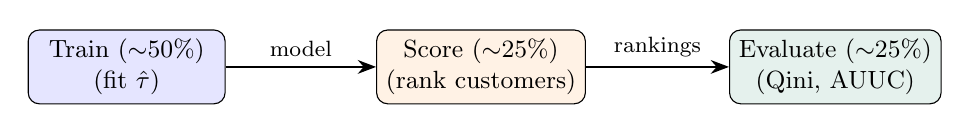
\begin{tikzpicture}[
    box/.style={draw, rounded corners, minimum width=2.5cm, minimum height=0.8cm, font=\small, align=center}
]
\node[box, fill=blue!10] (train) at (0,0) {Train ($\sim$50\%)\\(fit $\hat{\tau}$)};
\node[box, fill=orange!10] (score) at (4.5,0) {Score ($\sim$25\%)\\(rank customers)};
\node[box, fill=sbgreen!10] (eval) at (9,0) {Evaluate ($\sim$25\%)\\(Qini, AUUC)};
 
\draw[-{Stealth}, thick] (train) -- (score) node[midway, above, font=\footnotesize] {model};
\draw[-{Stealth}, thick] (score) -- (eval) node[midway, above, font=\footnotesize] {rankings};
\end{tikzpicture}
\end{center}
 
\bigskip
 
\textbf{Alternative: cross-fitting.} Partition into $K$ folds, train on $K-1$, produce out-of-fold scores, compute metrics on pooled predictions.
 
\bigskip
 
Uses all data for both estimation and evaluation while maintaining independence.
\end{frame}
 
% ====================================================================
\begin{frame}{The Full Pipeline}
 
\begin{center}
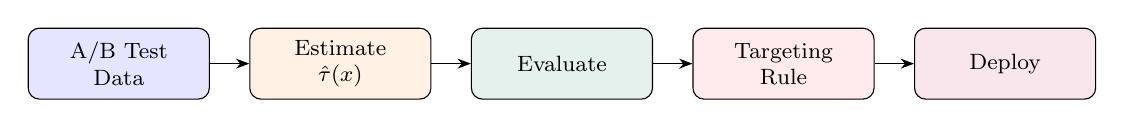
\begin{tikzpicture}[
    node distance=0.6cm and 0.5cm,
    box/.style={draw, rounded corners, minimum width=2.3cm, minimum height=0.9cm, font=\footnotesize, align=center},
]
\node[box, fill=blue!10] (data) {A/B Test\\Data};
\node[box, fill=orange!10, right=of data] (est) {Estimate\\$\hat{\tau}(x)$};
\node[box, fill=sbgreen!10, right=of est] (eval) {Evaluate};
\node[box, fill=red!8, right=of eval] (target) {Targeting\\Rule};
\node[box, fill=purple!10, right=of target] (deploy) {Deploy};
 
\draw[-{Stealth}] (data) -- (est);
\draw[-{Stealth}] (est) -- (eval);
\draw[-{Stealth}] (eval) -- (target);
\draw[-{Stealth}] (target) -- (deploy);
\end{tikzpicture}
\end{center}
 
\bigskip
 
\textbf{Estimate:} S-Learner, T-Learner, causal forest, \ldots
 
\textbf{Evaluate:} Ranking (Qini, AUUC, RATE), calibration, policy value.
 
\textbf{Target:} Threshold rule $\hat{\tau}(x_i) \cdot m > c$, or budget-constrained ranking.
 
\textbf{Deploy:} Score new customers, send coupons.
\end{frame}
 
% ====================================================================
\begin{frame}{Limitations to Keep in Mind}
 
\begin{enumerate}
    \item \textbf{AUUC doesn't tell you whether to treat.} It measures ranking, not whether the average effect justifies the cost.
 
    \medskip
 
    \item \textbf{Noisy at the extremes.} The left-hand side of the Qini curve (small top groups) is where targeting matters most and estimation is least reliable.
 
    \medskip
 
    \item \textbf{Sensitive to the share of ``movers.''} If 95\% of customers have near-zero CATEs, even a perfect model shows little AUUC.
 
    \medskip
 
    \item \textbf{Rankings, not mechanisms.} A model may rank well by exploiting a statistical artifact that does not generalize.
\end{enumerate}
\end{frame}
 
% ====================================================================
\begin{frame}{Key Takeaways}
 
\begin{enumerate}
    \item Individual treatment effects are \textbf{never observed}. Evaluate by targeting quality.
 
    \medskip
 
    \item The \textbf{Qini curve} plots incremental effect vs.\ fraction targeted. \textbf{AUUC} summarizes it.
 
    \medskip
 
    \item The \textbf{RATE} provides formal inference for model comparison.
 
    \medskip
 
    \item \textbf{Calibration} checks magnitudes. Good ranking $\neq$ good magnitudes.
 
    \medskip
 
    \item \textbf{Policy value} (AIPW) evaluates the deployed targeting rule directly.
 
    \medskip
 
    \item \textbf{Honest evaluation} requires sample splitting or cross-fitting.
 
    \medskip
 
    \item \textbf{Now: Lab.} Fit meta-learners, compute Qini curves, compare, build a targeting rule.
\end{enumerate}
\end{frame}
 

\end{document}
